\documentclass[conference]{IEEEtran}

\usepackage{graphicx}
\usepackage{amsmath}
\usepackage{booktabs}
\usepackage{multirow}
\usepackage{cite}
\usepackage{url}

\title{CardioM3Net: Multimodal Meta-Learning for ECG-PCG-Clinical Diagnosis}

% \author{\IEEEauthorblockN{Author Name}
% \IEEEauthorblockA{Department\\University\\Email}}

\begin{document}
\maketitle

\begin{abstract}
% TODO: 150--250 words. Summarize the model, datasets, and key results.
\end{abstract}

\begin{IEEEkeywords}
Multimodal learning; ECG; PCG; meta-learning; domain adaptation; cardiovascular disease.
\end{IEEEkeywords}

\section{Introduction}
% Motivation, problem statement, and contributions.

\section{Related Work}
% ECG/PCG fusion, meta-learning in healthcare, domain adaptation for ECG.

\section{Methods}
\subsection{Data Sources and Preprocessing}
% PTB-XL ECG, CinC 2016 PCG, UCI clinical tabular features.

\subsection{CardioM3Net Architecture}
% ECG encoder, PCG encoder, clinical encoder, fusion, multi-task heads.

\begin{figure}[t]
    \centering
    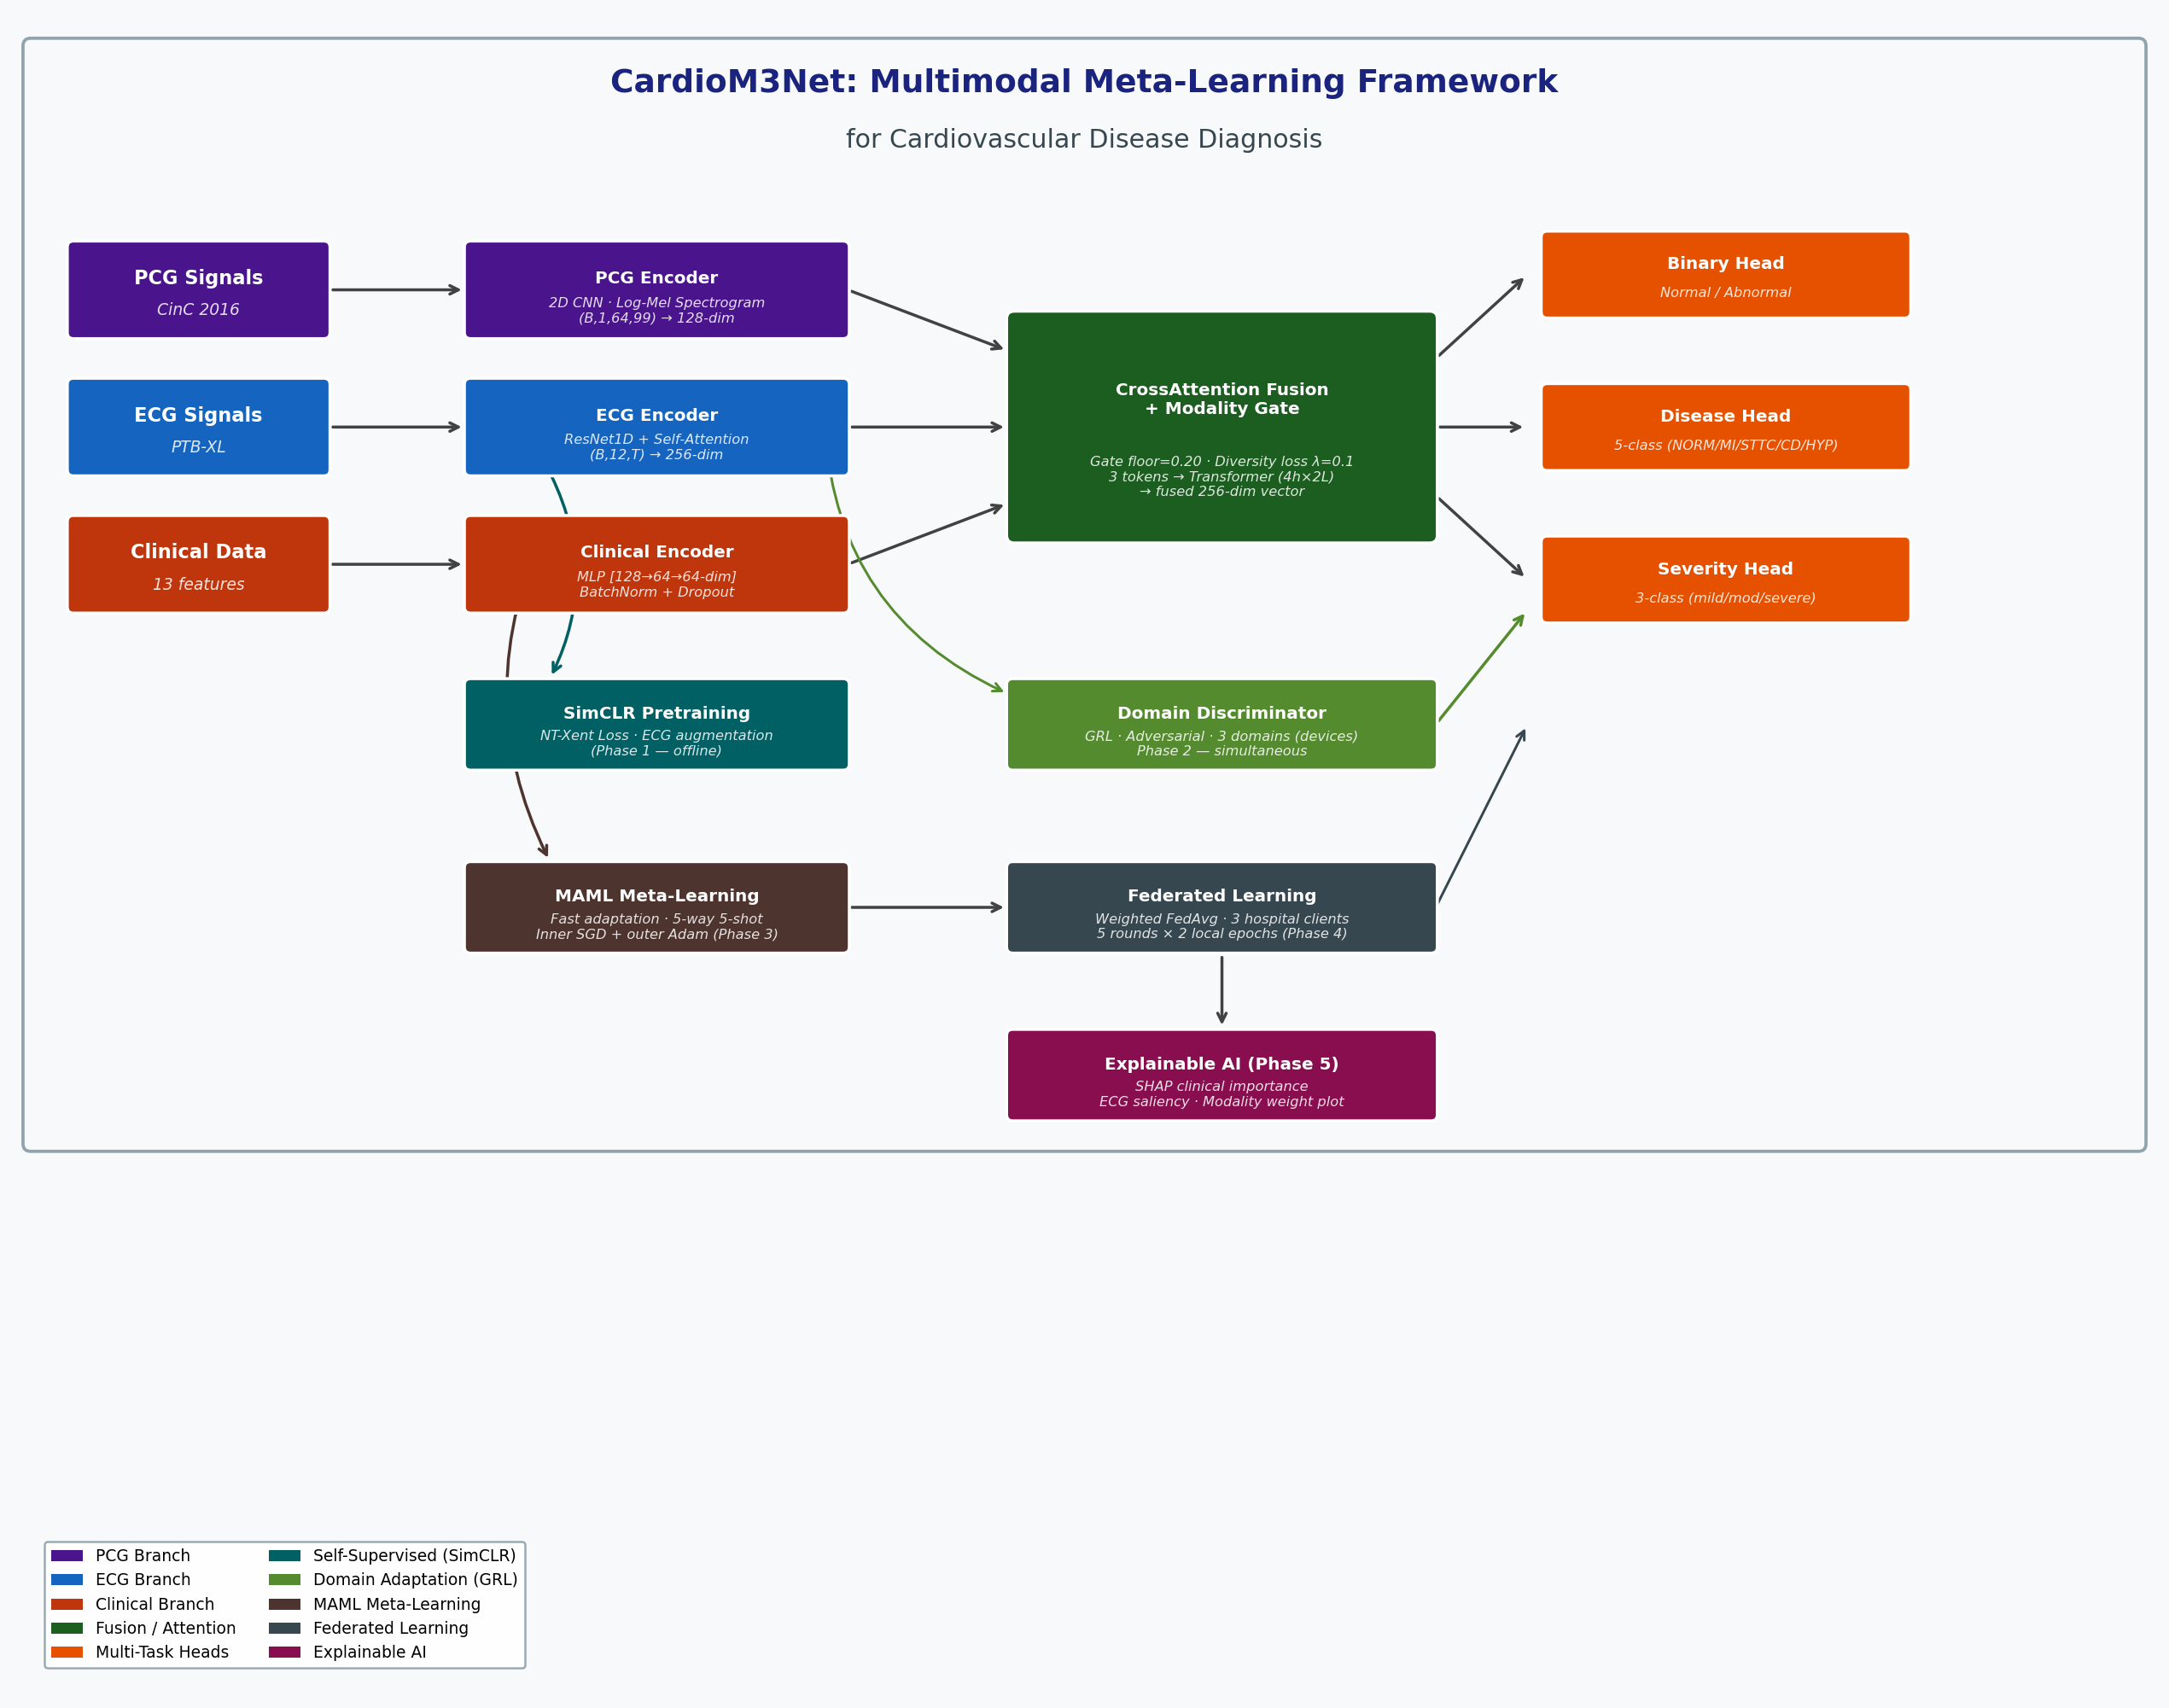
\includegraphics[width=\columnwidth]{../../cardiom3net_results/diagram1_architecture.png}
    \caption{Overall CardioM3Net architecture (ECG/PCG/clinical branches and fusion).}
    \label{fig:architecture}
\end{figure}

\subsection{Training Pipeline}
% Self-supervised pretraining, supervised multi-task, MAML, domain adaptation, federated (if included here).

\section{Experiments}
\subsection{Experimental Setup}
% Splits, evaluation metrics, training schedule.

\begin{table}[t]
\centering
\caption{Summary of datasets used in experiments.}
\label{tab:datasets}
\begin{tabular}{lccc}
\toprule
Dataset & Modality & Samples & Labels \\
\midrule
PTB-XL & ECG + clinical & --- & 5-class + severity \\
CinC 2016 & PCG & --- & Normal/abnormal \\
UCI Heart Disease & Clinical & --- & CVD risk \\
\bottomrule
\end{tabular}
\end{table}

\section{Results}
\subsection{Overall Performance}

\begin{figure}[t]
    \centering
    
\includegraphics[width=\columnwidth]{../../cardiom3net_results/roc_curves.png}
    \caption{Binary ROC curves for CardioM3Net variants (central and federated).}
    \label{fig:roc}
\end{figure}

\begin{figure}[t]
    \centering
    
\includegraphics[width=\columnwidth]{../../cardiom3net_results/precision_recall_curves.png}
    \caption{Precision-Recall curves for binary cardiac risk detection.}
    \label{fig:pr}
\end{figure}

\begin{figure}[t]
    \centering
    
\includegraphics[width=\columnwidth]{../../cardiom3net_results/per_class_roc.png}
    \caption{Per-class one-vs-rest ROC curves for the five disease categories (NORM, MI, STTC, CD, HYP).}
    \label{fig:per_class_roc}
\end{figure}

\begin{figure}[t]
    \centering
    
\includegraphics[width=\columnwidth]{../../cardiom3net_results/confusion_matrices.png}
    \caption{Confusion matrices for binary and five-class disease classification.}
    \label{fig:cm}
\end{figure}

\begin{figure}[t]
    \centering
    
\includegraphics[width=\columnwidth]{../../cardiom3net_results/confusion_matrix_normalized.png}
    \caption{Row-normalized confusion matrix showing per-class recall for disease classification.}
    \label{fig:cm_norm}
\end{figure}

\begin{figure}[t]
    \centering
    
\includegraphics[width=\columnwidth]{../../cardiom3net_results/class_metrics_radar.png}
    \caption{Radar charts of per-class precision, recall, and F1-score for the five disease categories.}
    \label{fig:radar}
\end{figure}

\begin{table}[t]
\centering
\caption{Performance metrics (to be filled from evaluation logs).}
\label{tab:metrics}
\begin{tabular}{lcccc}
\toprule
Task & Acc & F1 & AUC & Recall \\
\midrule
Normal vs Abnormal & --- & --- & --- & --- \\
Disease (5-class) & --- & --- & --- & --- \\
Severity (3-class) & --- & --- & --- & --- \\
\bottomrule
\end{tabular}
\end{table}

\subsection{Training Dynamics}
\begin{figure}[t]
    \centering
    
\includegraphics[width=\columnwidth]{../../cardiom3net_results/training_curves.png}
    \caption{Training curves across phases (self-supervised + supervised).}
    \label{fig:training}
\end{figure}

\begin{figure}[t]
    \centering
    
\includegraphics[width=\columnwidth]{../../cardiom3net_results/maml_loss.png}
    \caption{MAML meta-learning query loss per episode with moving-average smoothing.}
    \label{fig:maml}
\end{figure}

\subsection{Ablation Study}
\begin{figure}[t]
    \centering
    
\includegraphics[width=\columnwidth]{../../cardiom3net_results/model_comparison.png}
    \caption{Grouped bar chart comparing CardioM3Net against baseline models across all metrics.}
    \label{fig:ablation}
\end{figure}

\section{Discussion}
% Interpret results, error analysis, limitations.

\section{Conclusion}
% Summary and future work.

\section*{Acknowledgment}
% Optional.

\bibliographystyle{IEEEtran}
\bibliography{refs}

\end{document}
